\chapter{The Acuity Model}
\label{ch:acuity}

A blur radius alone is not the quantity a clinician, or an IYPT judge, ultimately cares
about: the relevant output is predicted \emph{visual acuity}, conventionally reported
in LogMAR (log Minimum Angle of Resolution) or Snellen notation. This project converts
the ASM-computed retinal blur into a LogMAR prediction via a specific, cited pipeline
implemented in \texttt{stage4\_human\_vision/acuity.py} (verified read directly).

\section{Why blur radius is the wrong optimization target on its own}
Minimizing a blur-radius metric directly (e.g.\ $r_{EE}(50\%)$) does not necessarily
minimize predicted acuity loss, because the mapping from blur to acuity is nonlinear and
itself depends on the eye's own optical transfer function and on retinal illuminance,
not on blur radius alone. \texttt{MASTER\_HANDBOOK.tex} Chapter~5 documents two
successive corrections made to an earlier, blur-radius-only optimization approach: first
an explicit brightness floor (Section~\ref{sec:brightness}), then optimizing acuity
directly rather than blur (used throughout this project's array-evaluation chapters).

\section{Pupil and retinal illuminance}
Retinal illuminance is computed from the light entering through the active aperture(s)
at a given gaze condition, scaled by scene luminance, and reported in trolands (Td),
the standard unit for retinal illuminance referenced to pupil area. This project's
default scene luminance is $10{,}000\,\mathrm{cd/m^2}$ (bright outdoor daylight), with
default field diameter $20^\circ$ and default observer age $28.58$ years (source:
\texttt{stage4\_human\_vision/config.py} defaults, \texttt{default\_scene\_luminance\_cdm2},
\texttt{default\_field\_diameter\_deg}, \texttt{default\_age\_years}; verified present).

\section{MTF, contrast sensitivity, and Visual Strehl}
The acuity predictor uses the aperture's actual modulation transfer function (MTF,
derived from the ASM-computed point spread function), evaluated against a contrast
sensitivity function (CSF) model, and a Visual Strehl ratio (VSOTF) -- the CSF-weighted
similarity of the actual optical transfer function to the diffraction-limited one --
as an overall optical-quality summary statistic. This is the same VSOTF/CSF machinery
discussed in detail, with a documented correction, in the array-level ghosting theory
(Section~\ref{sec:barten}); the acuity model here uses \texttt{stage3\_human\_vision}'s
own optical-quality and CSF evaluation directly, not a re-implementation.

\subsection{The recommended predictor}
\begin{align}
\mathrm{MAR}_{10} &= \frac{f_{20/20}}{f_{\mathrm{cutoff,10\%}}}
& \text{(MAR from the MTF's 10\% cutoff spatial frequency)} \\
\mathrm{MAR}_{\mathrm{VSOTF}} &= \frac{\mathrm{MAR}_{10}}{\mathrm{clip}(\mathrm{VSOTF},0.25,2.0)^{0.1}}
& \text{(Visual-Strehl adjustment)} \\
\mathrm{LogMAR}_{\mathrm{raw}} &= \log_{10}\!\big(\max(\mathrm{MAR}_{\mathrm{VSOTF}},10^{-6})\big)
\end{align}
This is the \texttt{mtf10\_vsotf\_brightness\_adjusted} model (source:
\texttt{stage4\_human\_vision/acuity.py}, function \texttt{predict\_acuity}, verified
read directly), the ``recommended'' model this project selects by configuration, not
chosen post-hoc per result.

A legacy alternative predictor (an uncited $\mathrm{SNR}^{0.05}$ correction term, in the
same file, function argument \texttt{legacy\_mar}) is retained in the codebase for
direct comparison, per this project's own stated design principle of keeping
alternative models available rather than silently deleting a superseded one
(\texttt{DESIGN.md}, cited in \texttt{acuity.py}'s own module docstring).

\begin{figure}[htbp]
\centering
\begin{minipage}{0.23\textwidth}\centering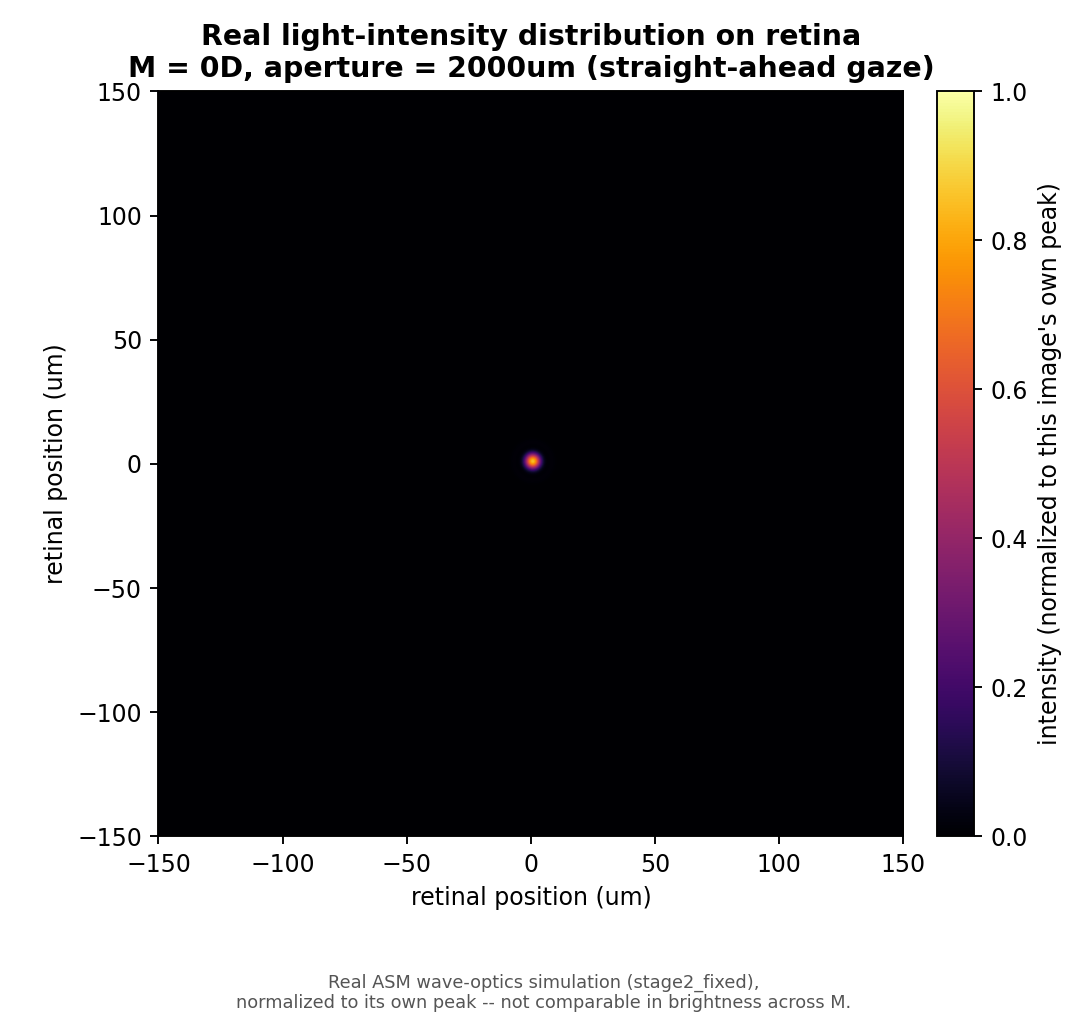
\includegraphics[width=\textwidth]{figures/realistic_heatmap_M0.png}\end{minipage}
\begin{minipage}{0.23\textwidth}\centering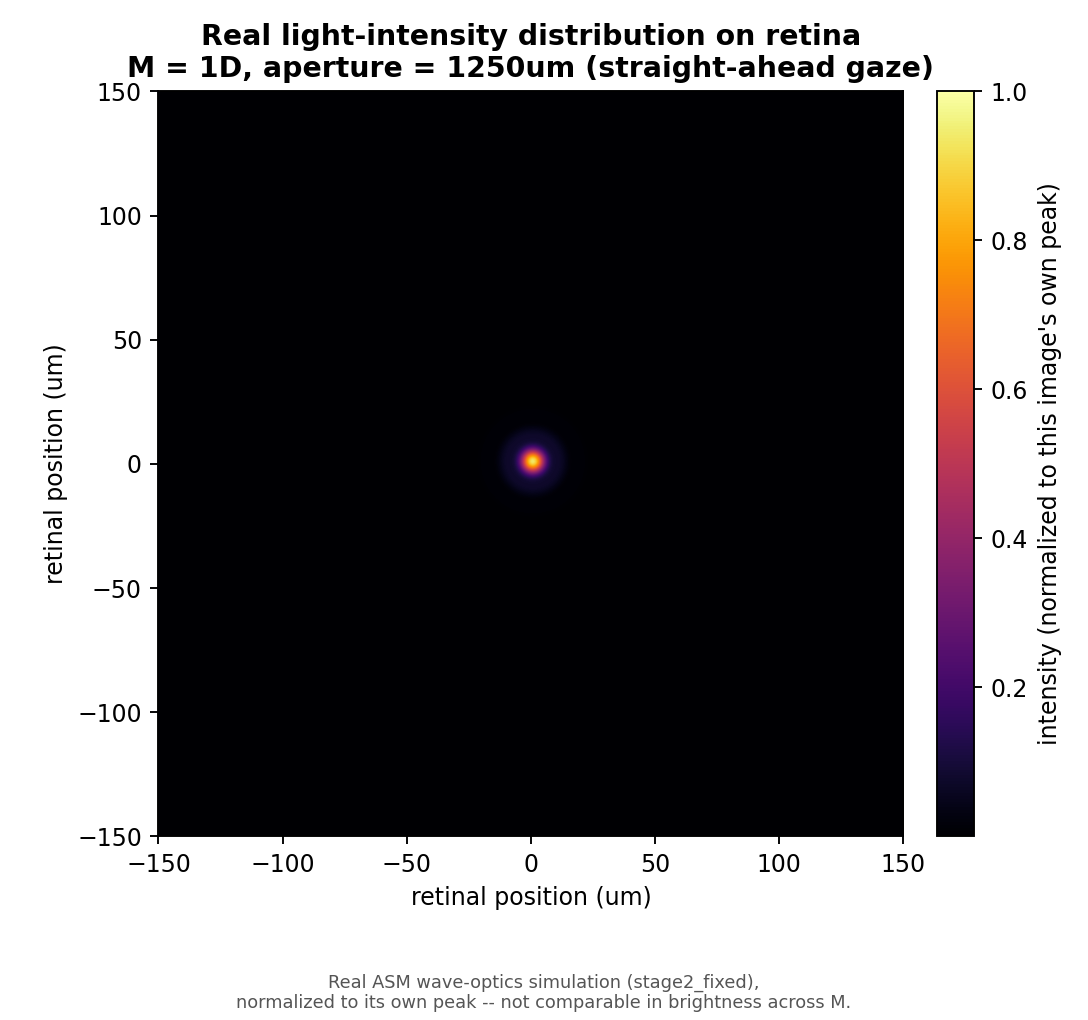
\includegraphics[width=\textwidth]{figures/realistic_heatmap_M1.png}\end{minipage}
\begin{minipage}{0.23\textwidth}\centering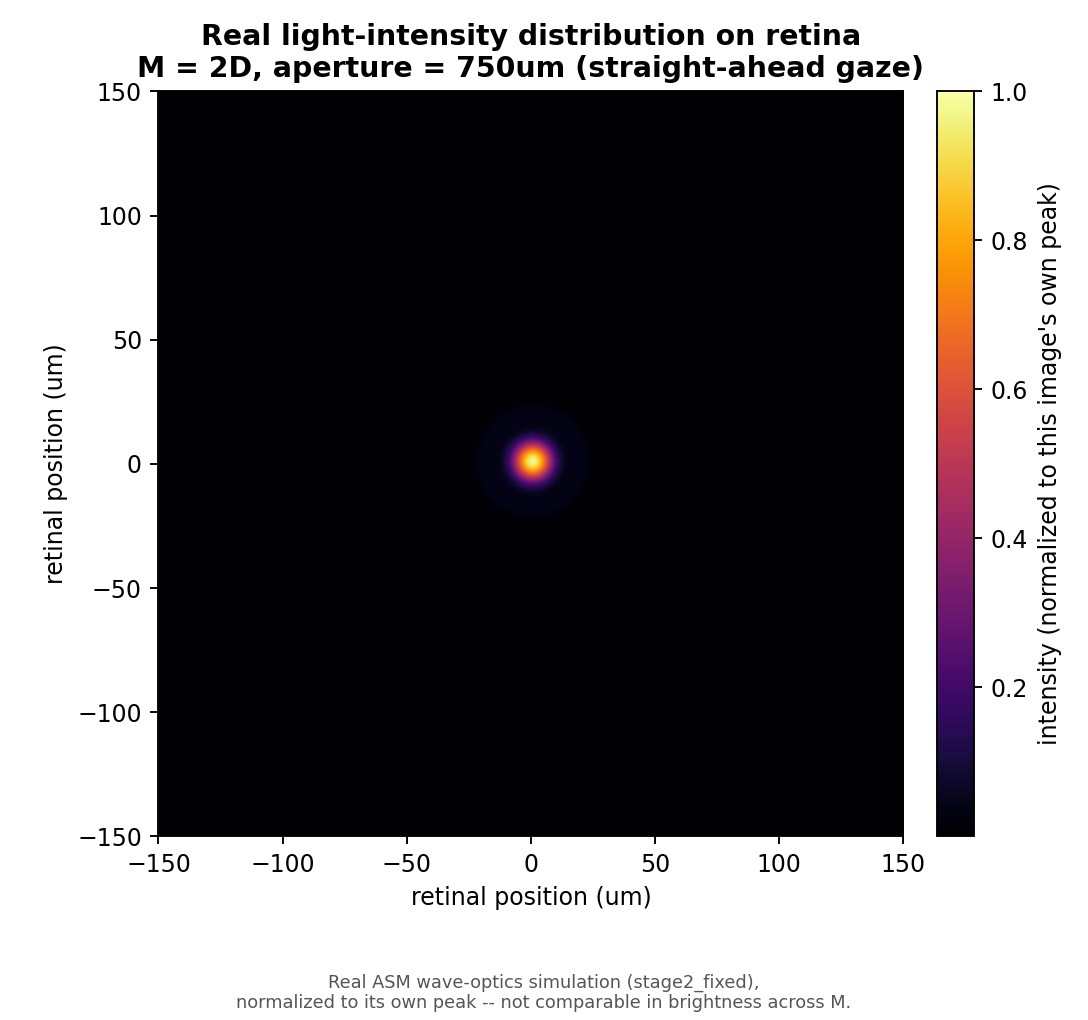
\includegraphics[width=\textwidth]{figures/realistic_heatmap_M2.png}\end{minipage}
\begin{minipage}{0.23\textwidth}\centering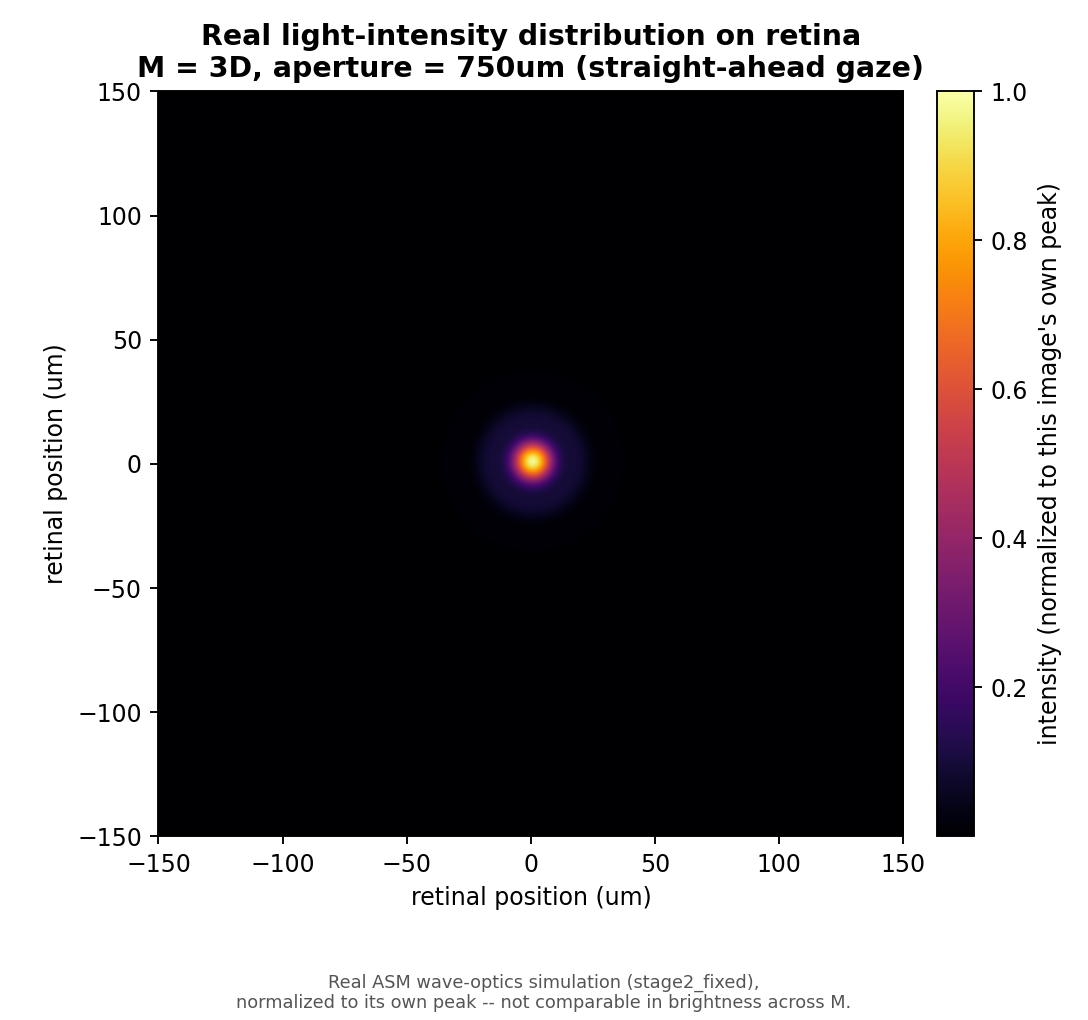
\includegraphics[width=\textwidth]{figures/realistic_heatmap_M3.png}\end{minipage}

\vspace{4pt}
\begin{minipage}{0.23\textwidth}\centering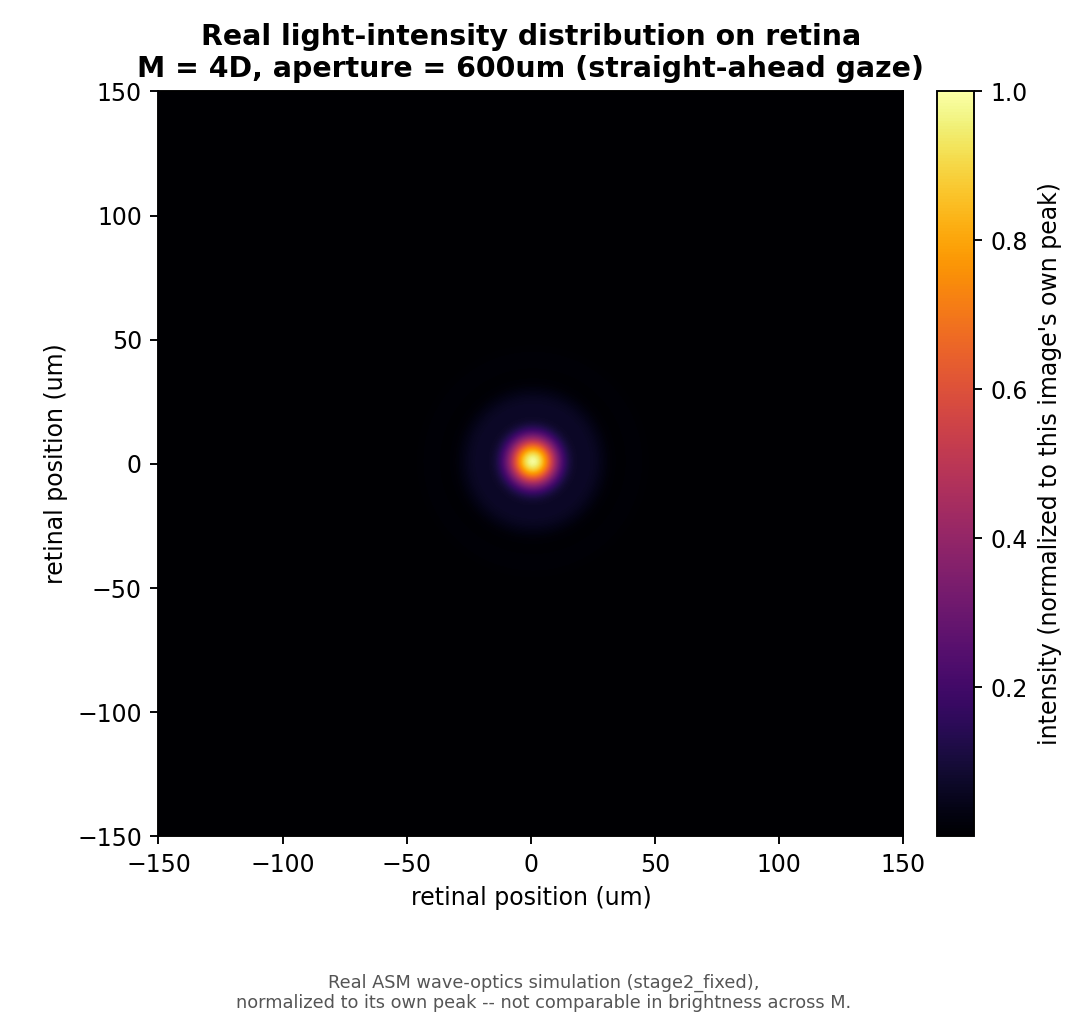
\includegraphics[width=\textwidth]{figures/realistic_heatmap_M4.png}\end{minipage}
\begin{minipage}{0.23\textwidth}\centering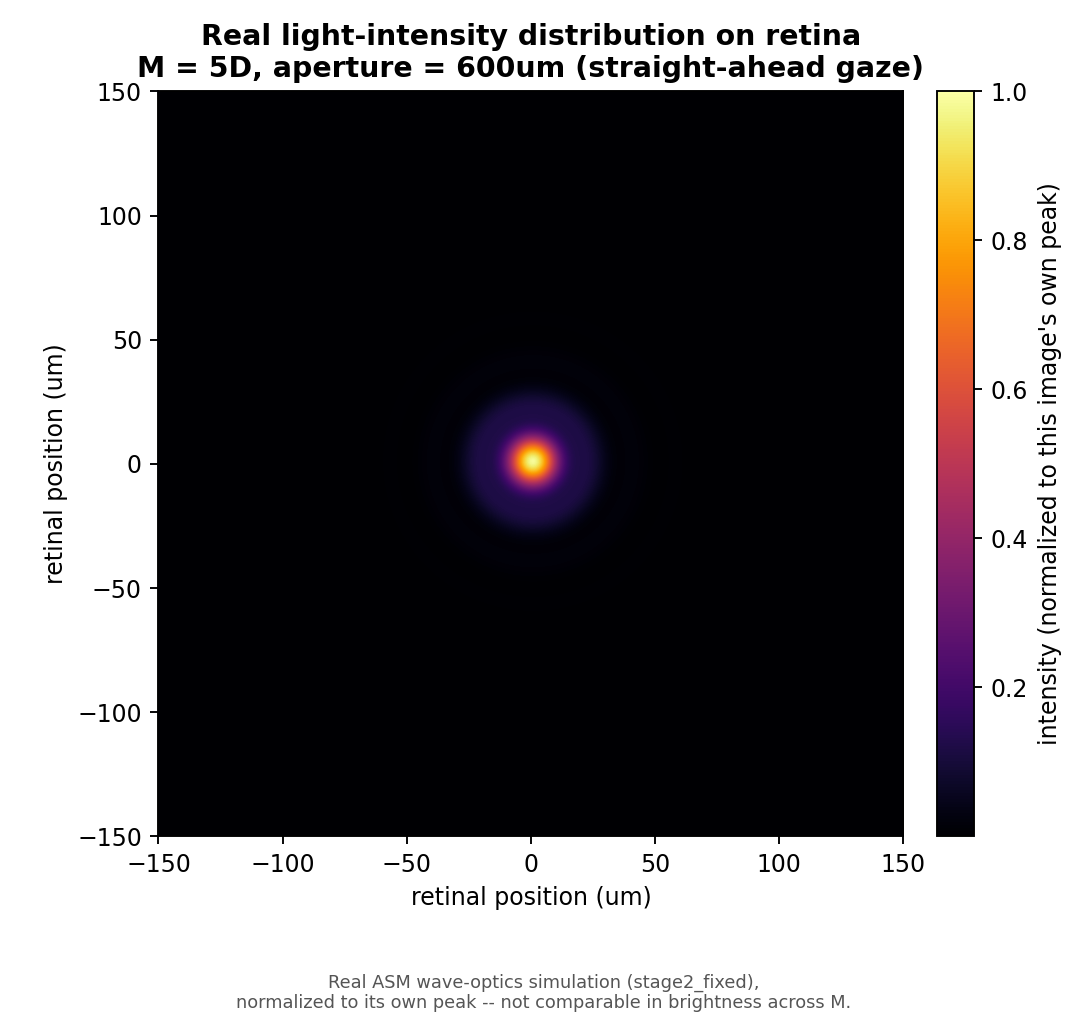
\includegraphics[width=\textwidth]{figures/realistic_heatmap_M5.png}\end{minipage}
\begin{minipage}{0.23\textwidth}\centering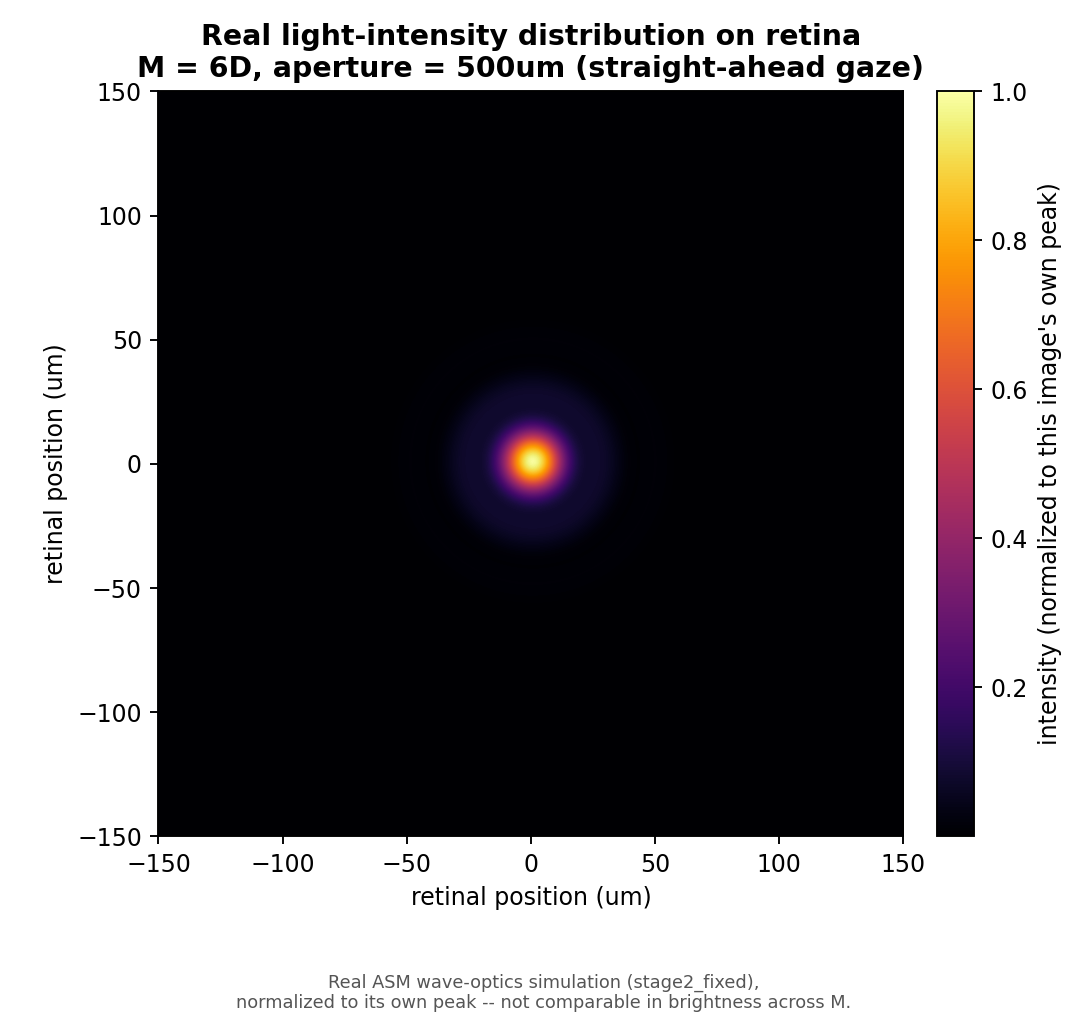
\includegraphics[width=\textwidth]{figures/realistic_heatmap_M6.png}\end{minipage}
\begin{minipage}{0.23\textwidth}\centering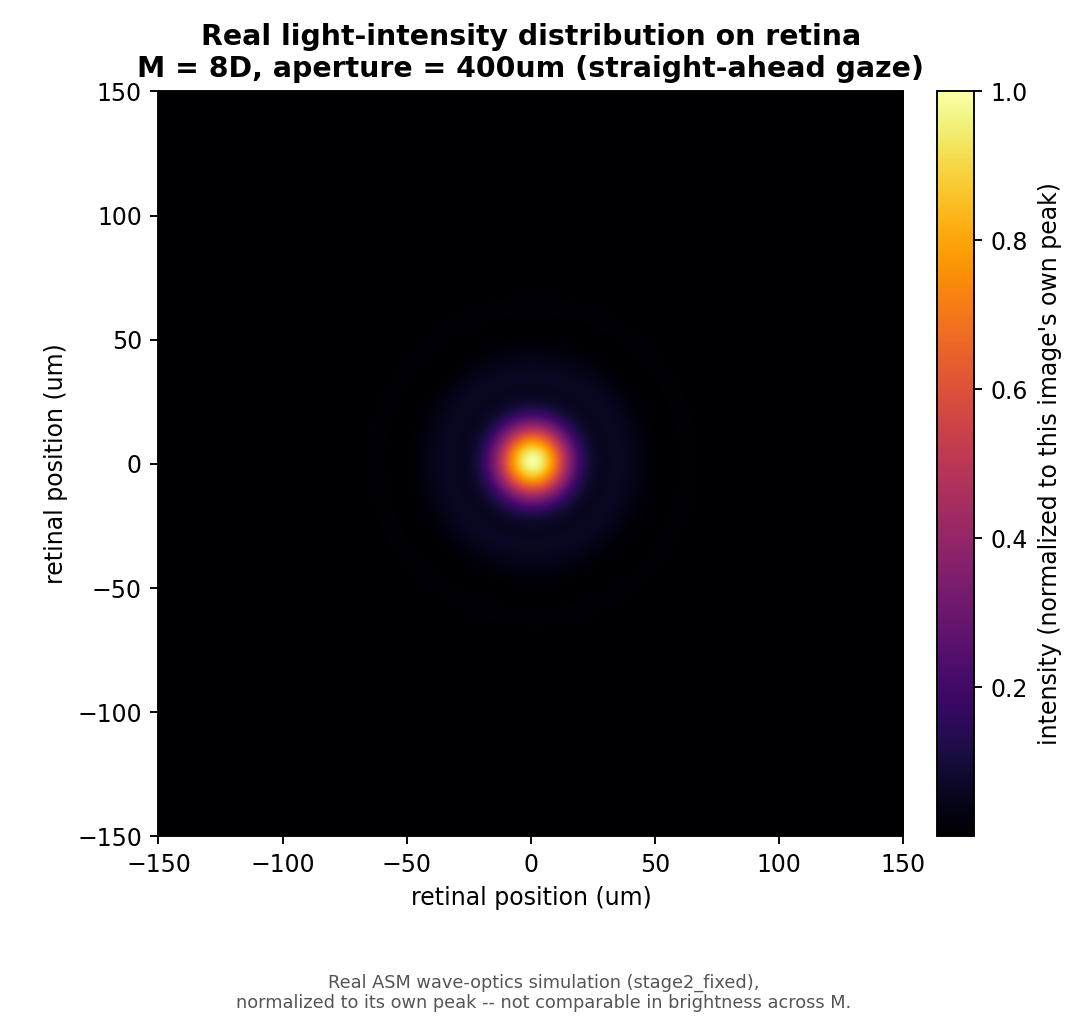
\includegraphics[width=\textwidth]{figures/realistic_heatmap_M8.png}\end{minipage}
\caption{Real retinal-plane intensity ($I_{\mathrm{retina}}=|U_{\mathrm{retina}}|^2$,
straight-ahead gaze) for all eight modeled myopia powers, left to right:
$M=0,1,2,3$D (top row), $M=4,5,6,8$D (bottom row), each at that $M$'s real
\texttt{PRIMARY\_WINNER\_PER\_M.csv} aperture. Every panel is the actual ASM
wave-optics output, not a schematic -- the growing blur radius from $M{=}0$ to
$M{=}8$ visible here is the same physical quantity the LogMAR curve above is
predicting a number for. Source:
\texttt{Array\_Design/array\_geometry\_lab/retinal\_light\_distribution\_simulation/}
\texttt{realistic\_heatmaps/realistic\_heatmap\_M\{0,1,2,3,4,5,6,8\}.png}, all eight
generated 2026-09-28 11:15--11:16 (verified via \texttt{stat}); each panel
normalized to its own peak, not comparable in absolute brightness across $M$
(Section~\ref{sec:limitations-optics}).}
\label{fig:retinal-grid-all-M}
\end{figure}

\section{The brightness correction}
\label{sec:brightness}
An additive LogMAR penalty is applied in the log domain for retinal illuminance below a
literature-cited knee:
\begin{equation}
\Delta\mathrm{LogMAR}_{\mathrm{brightness}} =
\begin{cases}
0 & E_{\mathrm{td}} \ge E_{\mathrm{knee}} \\[4pt]
s \cdot \log_{10}\!\left(\dfrac{E_{\mathrm{knee}}}{E_{\mathrm{td}}}\right) &
E_{\mathrm{td}} < E_{\mathrm{knee}}
\end{cases}
\label{eq:brightness}
\end{equation}
with knee $E_{\mathrm{knee}}=300$\,Td and slope $s=0.060$ LogMAR per log$_{10}$-unit of
illuminance (source: \texttt{stage4\_human\_vision/acuity.py},
\texttt{brightness\_logmar\_correction}, verified read directly).

\textbf{Knee value (300\,Td)}: cited to Van Nes \& Bouman (1967) \citep{vannes1967} --
threshold modulation (contrast sensitivity) is illuminance-\emph{independent}
(Weber--Fechner behaviour) above 300\,Td, and increases as $E_{\mathrm{td}}^{-1/2}$
(de~Vries--Rose behaviour) below it. Verified directly against the primary abstract per
this project's own citation-verification discipline (\texttt{stage4\_human\_vision/literature.py}).

\textbf{Slope (0.060 LogMAR/log$_{10}$-unit)}: cited to Tidbury, Czanner \& Newsham
(2016), verified directly against the full text (their Table 3, $p<0.001$), and
cross-checked (not directly used) against Sheedy, Bailey \& Raasch (1984)'s
independently-derived value of $\approx0.0664$, which could only be verified against a
secondary summary rather than the primary source -- the directly-verified Tidbury value
is the one used, per this project's stated preference for primary-source-verified
citations over secondary ones of comparable magnitude.

Rabin (1994) is cited as independent corroboration of the qualitative direction of this
effect (visual acuity is considerably \emph{more} resistant to reduced luminance than
contrast sensitivity is, in the photopic range they tested: a $116\to0.23\,\mathrm{cd/m^2}$
reduction gave a $3\times$ acuity loss against a $17\times$ contrast-sensitivity loss)
-- but the exact numerical knee and slope used in Equation~\ref{eq:brightness} come from
Van Nes \& Bouman and Tidbury et al.\ respectively, both natively reported in the units
this equation needs (trolands, LogMAR), not from Rabin's own cd/m$^2$-based data.

Every design evaluated in this project's array chapters (Chapters~\ref{ch:model-a},
\ref{ch:model-b}) sits well above the 300\,Td knee at the default $10{,}000\,\mathrm{cd/m^2}$
scene luminance; the brightness term is therefore \textbf{inert (zero)} for every
reported result in this paper, and is documented here in full for completeness and
falsifiability, not because it changes any headline number.

\section{Full acuity-model input inventory}
\begin{center}
\begin{tabular}{lll}
\toprule
Input & Default value & Source \\
\midrule
Scene luminance & $10{,}000\,\mathrm{cd/m^2}$ & \texttt{config.py} \\
Field diameter & $20^\circ$ & \texttt{config.py} \\
Observer age & $28.58$ years & \texttt{config.py} \\
Pupil diameter & $4000\,\mu$m & project-wide constant \\
ASM grid resolution & $4096$ (post-fix, Section~\ref{sec:gridN}) & \texttt{run\_acuity\_sweep.py} \\
Wavelength & 550\,nm (vacuum) & \texttt{run\_acuity\_sweep.py} \\
Spectacle gap & 12\,mm & \texttt{run\_acuity\_sweep.py} \\
\bottomrule
\end{tabular}
\end{center}
